\documentclass[12pt, a4paper]{article}
\setlength{\textheight}{24cm}
\setlength{\textwidth}{16cm}
\setlength{\topmargin}{0cm}
\setlength{\evensidemargin}{0cm}
\setlength{\oddsidemargin}{0cm}
\usepackage[affil-it]{authblk}
\usepackage{graphics}
\usepackage{graphicx}
\usepackage{caption}
\usepackage{float}
\usepackage[british]{babel}
\usepackage{hyperref}
\usepackage{subcaption}
\date{}
\begin{document}
\title{Comparison of Several Frameworks for General-Purpose Programming and the  Computation of FFTs on GPUs}
\author{Philippe Gambron \thanks{\texttt{philippe.gambron{@}stfc.ac.uk}}, Sue Thorne \thanks{\texttt{sue.thorne{@}stfc.ac.uk}}}
\affil{Science and Technology Facilities Council, Hartree Centre, Rutherford Appleton Laboratory, Harwell Campus, Harwell Oxford, OX11 0QZ, United Kingdom}
\date{\today}
\maketitle
\begin{abstract}
We compare the performance of several GPU frameworks that can be used,
in C or C++, for general-purpose programming or computing Fast Fourier
Transforms using the available GPU. The frameworks considered are
CUCA, OpenCL, OpenACC, OpenMP and Kokkos.
\end{abstract}


\section{Introduction}
During the last decade, the use of graphical processing units (GPUs)
has become increasingly widespread.  While there are some overheads
associated with data transfers and some constraints
on the types of algorithms can be efficiently programmed, one can
obtain tremendous performance gains on suitable problems.

In this report, we compare the performances obtained with a number of
frameworks that have been developed to allow software to use GPUs.
Within our benchmark tests, we use a simple general-purpose programming
example and also compute Fast Fourier Transforms (FFT) on the GPU by
using the FFT libraries provided by some of these frameworks.

\subsection{Overview of the chosen frameworks}
We consider the following frameworks for GPU programming: CUDA
\cite{cuda}, OpenCL \cite{opencl}, \mbox{OpenACC} \cite{openacc},
OpenMP \cite{openmp}\footnote{From version 4.0, OpenMP offers GPU
  programming capabilities.} and Kokkos \cite{kokkos}. The first three
of these frameworks also provide FFT libraries, which are cuFFT
\cite{cufft}, clFFT \cite{clfft} and AccFFT \cite{accfft},
respectively. Table \ref{ffttable} contains an overview of their
properties. They can perform complex, real-to-half-complex
and half complex-to-real transforms. The half-complex output
consists of half as many complex values as there were points in the
signal, taking advantage of the hermiticity of the Fourier transform
of a real function.

\begin{table}[H]
\captionsetup{width=0.8\textwidth}
\centering
\begin{tabular}{|p{2.5cm}||p{2.5cm}|p{1cm}|p{3cm}|p{3cm}|p{2cm}|p{2cm}|}
\hline
& Type & Dim. & Radices & Licence \\
\hline
\hline
AccFFT & R$\to$H,\ \ \  C$\to$C& 3& & GPL v2\\
\hline
clFFT  &  R$\to$H,\ \ \  C$\to$C,\ \ \ \  H$\to$R& 1, 2, 3 & 2, 3, 5, 7 & Proprietary\\
\hline
cuFFT  &  R$\to$H,\ \ \  C$\to$C,\ \ \ \  H$\to$R & 1, 2, 3 & 2, 3, 5, 7 & GPL v3\\
\hline
\end{tabular}
\caption{Overview of the FFT libraries considered. R stands for real, C for complex and HC for half-complex.}
\label{ffttable}
\end{table}

\section{Benchmark}
The benchmark\footnote{The source code is available at:
  \hyperlink{https://github.com/SoftwareOutlook/GPU}{https://github.com/SoftwareOutlook/GPU}.}
consists of the processing a real or complex signal on a domain in 1,
2 or 3 dimensions. We first multiply it by a series of real signals,
thus producing another series of real or complex signals, and then
take their FFT.  The purpose was to mimick a problem submitted by the
CCP PET-MR collaboration \cite{ccppetmr} to us, the Software Outlook
initiative \cite{softwareoutlook}, that requires the multiplication of
a complex image by a series of coil sensitivities and then computing
the FFT of these products. In Section \ref{PRODUCT}, we benchmark the
multiplication of th eimages by coil sensitivites, while, in Section
\ref{FFT}, we study the performance obtained while computing the
FFT. For the example specific to the CCP/PET-MR collaboration (Section
\ref{CCPPETMR}), we take the FFT of 32 square images. In the more
general case, we use a single signal but consider domains in 1, 2 or 3
dimensions. The benchmark is depicted in Figure~\ref{benchmark} and
described more extensively in \cite{FFTREPORT}.

\begin{figure}[H]
\captionsetup{width=0.6\textwidth}
\centering
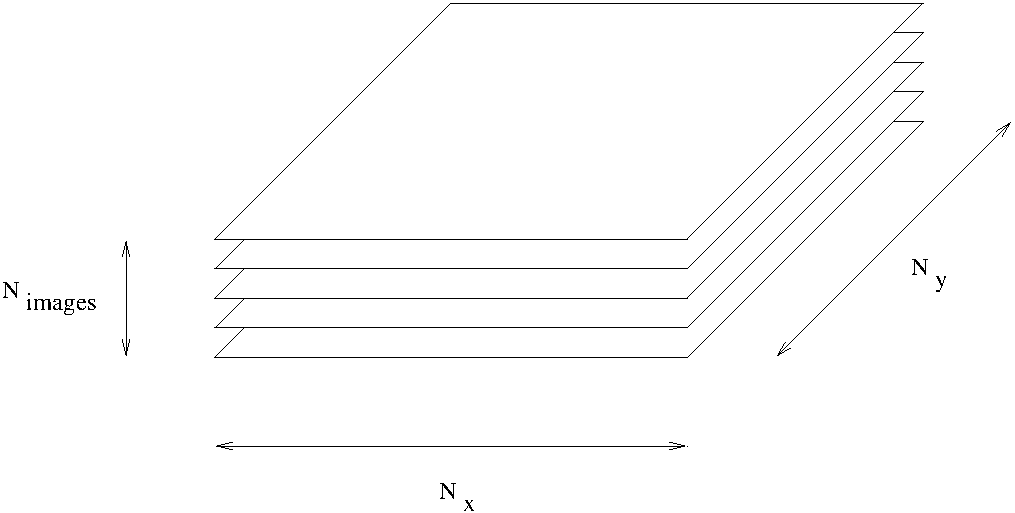
\includegraphics[height=5cm]{benchmark.pdf}
\caption{The benchmark consists in taking the FFT of several images. Each of them is made of real or complex values and can be a simple line, a rectangle or a cuboid.}
\label{benchmark}
\end{figure}

The
values appearing in the graphs are the wallclock initialisation and FFT execution
times averaged over 10 runs. There are some bumps in the graphs, which
are consistently seen when we repeat the measurements.

\subsection{Testing Environment Setup}

The measurements were carried out on a system featuring an Intel Xeon
W-2133 CPU (6 cores, 3.6 GHz), a NVIDIA Quadro GV100 GPU and 12 GB of
RAM. We used GCC compiler (version 7.3.0) with the following frameworks:
\begin{itemize}
 \item OpenCL version 1.2.7,
 \item OpenACC version 2.7,
 \item OpenMP version 4.0.0,
 \item Kokkos version 2.9.0,
 \item clFFT version 2.0,
\end{itemize}
and the NVCC compiler (version 10.0.130), which used the above version
of GCC as its host compiler with the following framework:
\begin{itemize}
\item CUDA version 10.0.130.
\end{itemize}


In this context, one disadvantage of OpenCL becomes
apparent: the support for it is more limited due to the most recent versions
(from 2.0 onwards) being not completely supported by NVIDIA GPUs.

\section{Product}\label{PRODUCT}
In this section, we compare the multiplication of a 1D array of $2^{24}$ real or
complex numbers by an array of real numbers by considering the
operations executed in a serial way on the processor, in a
multi-threaded way using six cores with either OpenMP and Kokkos, or
on the GPU using CUDA, OpenCL, OpenACC, OpenMP and Kokkos. In the case
of CUDA and OpenCL, we have also included a comparison using streams or
queues, respectively. This is a mechanism that allows the concurrent execution of
kernels as well as overlapping data transfers in different directions.
\begin{figure}[H]
\captionsetup{width=0.8\linewidth}
\centering
\begin{subfigure}{.5\textwidth}
\centering
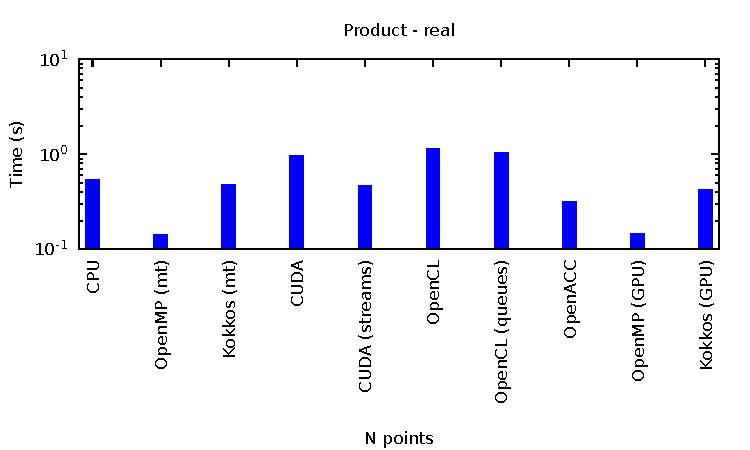
\includegraphics[width=.9\linewidth]{graphs/product-r.pdf}
\caption{Real}
\label{PRODR}
\end{subfigure}%
\begin{subfigure}{.5\textwidth}
\centering
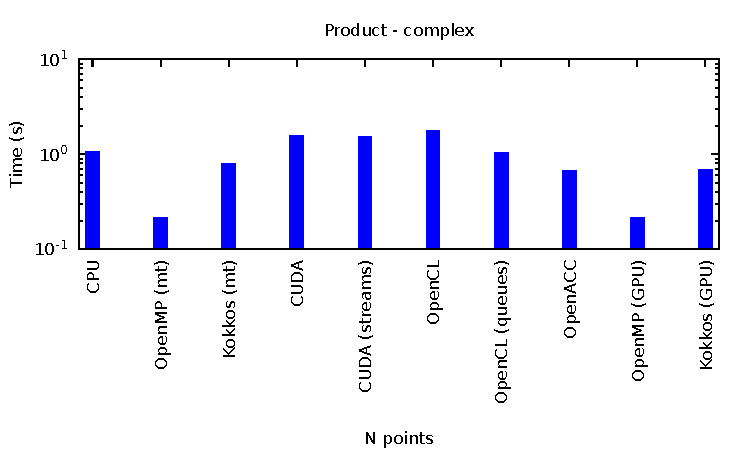
\includegraphics[width=.9\linewidth]{graphs/product-c.pdf}
\caption{Complex}
\label{PRODC}
\end{subfigure}
\caption{Execution time for the product of a large number of $2^{24}$ real and complex points using several frameworks.}
\label{1DFFTW}
\end{figure}

We observe that the best performance is obtained with OpenMP, both on
the CPU and the GPU. We note that, while compiling the example
involving Kokkos was straightforward, enabling CUDA required a
compilation that was more complicated\footnote{An external makefile as
  well as a header file containing the configuration must be
  included. This will produce, during compilation, several object
  files in the current directory that will have to be linked to
  produce our executable file. See \cite{KOKKOSDOC} for details. The
  environment variable \texttt{OMP\_PROC\_BIND} had also to be set to
  \texttt{spread} before the execution of the program.}.

\section{Fast Fourier Transform}\label{FFT}
We repeat the analysis carried out in \cite{FFTREPORT}. We measure the
wallclock initialisation and execution times obtained by computing the
FFT transform with cuFFT, clFFT and AccFFT for signals that were real
and complex in one, two and three dimensions. We initially consider
domains whose sides are identical and that contain a number of points
varying from $\sim 10^3$ to $\sim 10^8$.

Before we study in detail the performance obtained with GPUs, it is
enlightening to illustrate the effect they can provide by comparing
the performance obtained with cuFFT with the one achieved with FFTW
running in a serial way on the CPU. We have carried out these
measurements by computing the FFT of real and complex signals, in one
dimension. For a large number of points, the GPU improves the
performance by almost an order of magnitude while it is slower for a
small number of points because of the overheads (Figure
\ref{COMPGPUCPU}).
\begin{figure}[H]
\captionsetup{width=0.8\linewidth}
\centering
\begin{subfigure}{.5\textwidth}
\centering
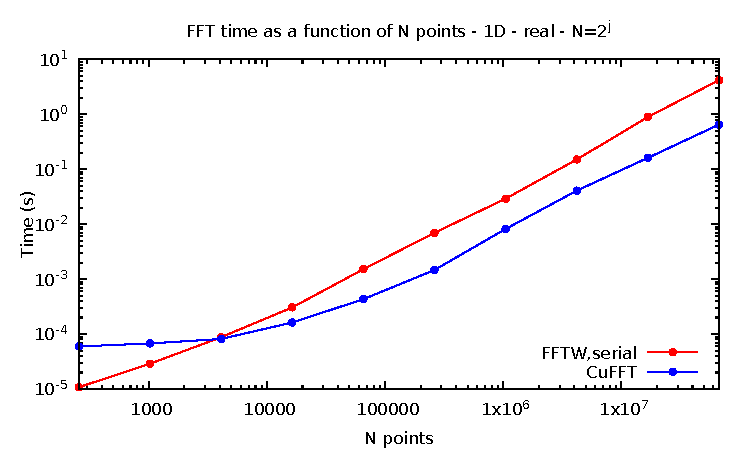
\includegraphics[width=.9\linewidth]{graphs/gpucpucomparison-r.pdf}
\caption{Real}
\label{GPUCPUR}
\end{subfigure}%
\begin{subfigure}{.5\textwidth}
\centering
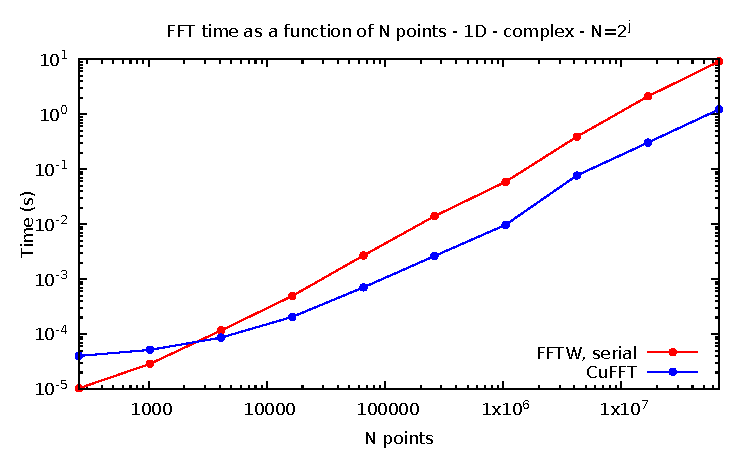
\includegraphics[width=.9\linewidth]{graphs/gpucpucomparison-c.pdf}
\caption{Complex}
\label{GPUCPUC}
\end{subfigure}
\caption{Comparison between the execution times obtained with cuFFT and FFTW running in a serial way on the CPU.}
\label{COMPGPUCPU}
\end{figure}


\subsection{Effect of the domain size in one dimension}\label{PERFORMANCE1D}
We compare the performance of the cuFFT, clFFT and AccFFT libraries in
Figures~\ref{FFTPOW21D} and \ref{FFT1D}. The lengths of the input
signal arrays that were used in these benchmarks are provided in
Table~\ref{1DSIZES}.


\begin{table}[H]
\centering
\begin{tabular}{|l|l|l|}
  \hline
  \multicolumn{3}{|c|}{$N_x$}\\
  \hline
  \hline
Powers of 2 & prod. pow. int. & primes\\ \hline
$2^8=256$ & $2\times 3\times 5\times 7 = 210$	& 257 \\ \hline
$2^{10}=1024$ & $2^2\times 3^2\times 5\times 7 = 1260$ & 1021 \\ \hline
$2^{12}=4096$ & $2^2\times 3^3\times 5\times 7 = 4410$ & 4093 \\ \hline
$2^{14}=16384$ & $2\times 3^2\times 5^3\times 7=15750$ & 16381 \\ \hline
$2^{16}=65536$ & $2\times 3^3\times 5^5\times 7^2 = 66150$ & 65521 \\ \hline
$2^{18}=262144$ & $2\times 3\times 5^3\times 7^3 = 257250$ & 262139 \\ \hline
$2^{20}=1048576$ & $2\times 3\times 5^2\times 7^4 = 1080450$ & 1048573 \\ \hline
$2^{22}=4194304$ & $2^3\times 3^2\times 5^2\times 7^4 = 4321800$ & 4194301 \\ \hline
$2^{24}=16777216$ & $2^3\times 3^2\times 5^4\times 7^3 = 15435000$ & 16777213 \\ \hline
$2^{26}=67108864$ & $2^3\times 3^3\times  5^3\times  7^4 = 64827000$ & 67108859 \\ \hline
\end{tabular}
\caption{Number of points used for the benchmark in one dimension}\label{1DSIZES}
\end{table}

The best FFT performance is obtained with cuFFT and, to a lesser
extent, clFFT. However the latter suffers from a drawback: its
initialisation time stays roughly constant no matter the problem size
and, for the smaller problem sizes, this initialisation time can the
between 2 and 3 orders of magnitude larger than the other libraries.
We also observe that, for small numbers of points, the performance
tends to be better for powers of 2, than for products of small
integers and finally for prime numbers.
  



\begin{figure}[H]
\captionsetup{width=0.8\linewidth}
\centering
\begin{subfigure}{.5\textwidth}
\centering
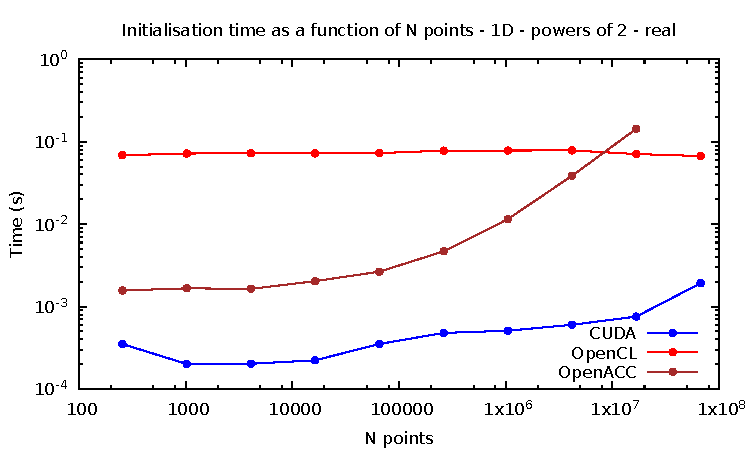
\includegraphics[width=.9\linewidth]{graphs/fft-1d-pow2-r-init.pdf}
\caption{Intialisation (real)}
\label{FFTPOW21DRI}
\end{subfigure}%
\begin{subfigure}{.5\textwidth}
\centering
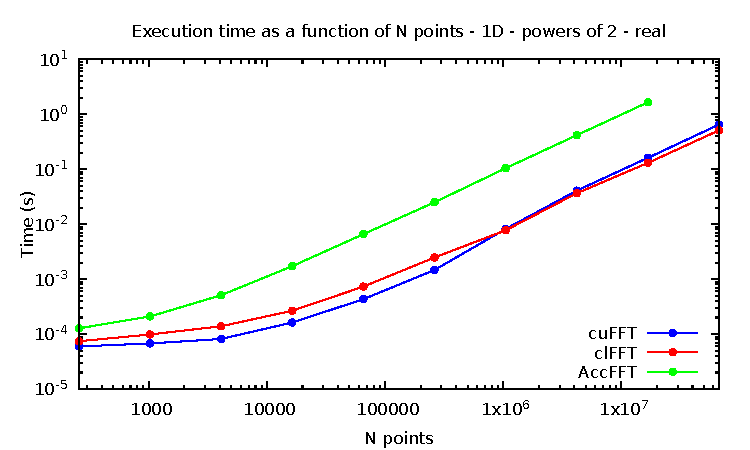
\includegraphics[width=.9\linewidth]{graphs/fft-1d-pow2-r-exec.pdf}
\caption{Execution (real)}
\label{FFTPOW21DRE}
\end{subfigure}\\
\begin{subfigure}{.5\textwidth}
\centering
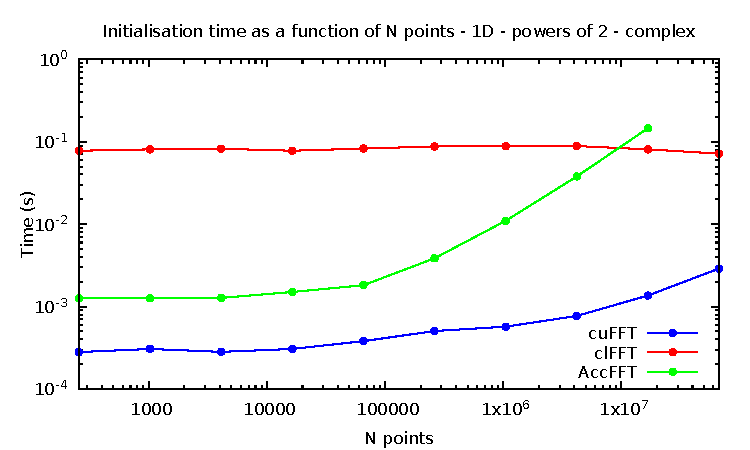
\includegraphics[width=.9\linewidth]{graphs/fft-1d-pow2-c-init.pdf}
\caption{Intialisation (complex)}
\label{FFTPOW21DCI}
\end{subfigure}%
\begin{subfigure}{.5\textwidth}
\centering
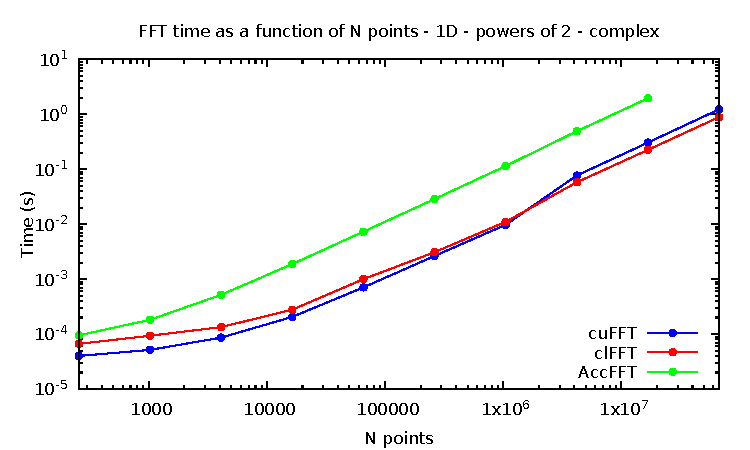
\includegraphics[width=.9\linewidth]{graphs/fft-1d-pow2-c-exec.pdf}
\caption{Execution (complex)}
\label{FFTPOW21DCE}
\end{subfigure}
\caption{Initialisation and execution times as a function of the number of points (1 dimension, powers of 2)}
\label{FFTPOW21D}
\end{figure}


\begin{figure}[H]
\captionsetup{width=0.8\linewidth}
\centering
\begin{subfigure}{.5\textwidth}
\centering
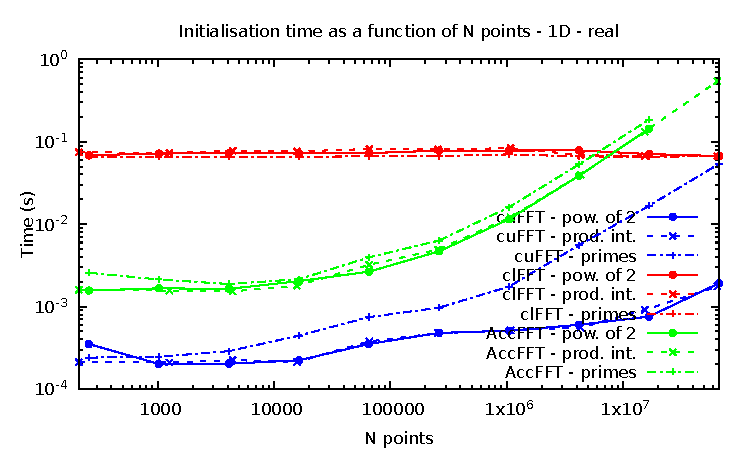
\includegraphics[width=.9\linewidth]{graphs/fft-1d-r-init.pdf}
\caption{Intialisation (real)}
\label{FFT1DRI}
\end{subfigure}%
\begin{subfigure}{.5\textwidth}
\centering
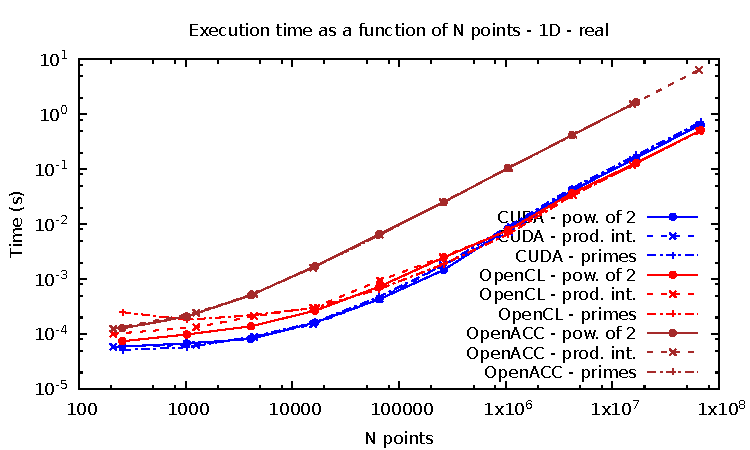
\includegraphics[width=.9\linewidth]{graphs/fft-1d-r-exec.pdf}
\caption{Execution (real)}
\label{FFT1DRE}
\end{subfigure}\\
\begin{subfigure}{.5\textwidth}
\centering
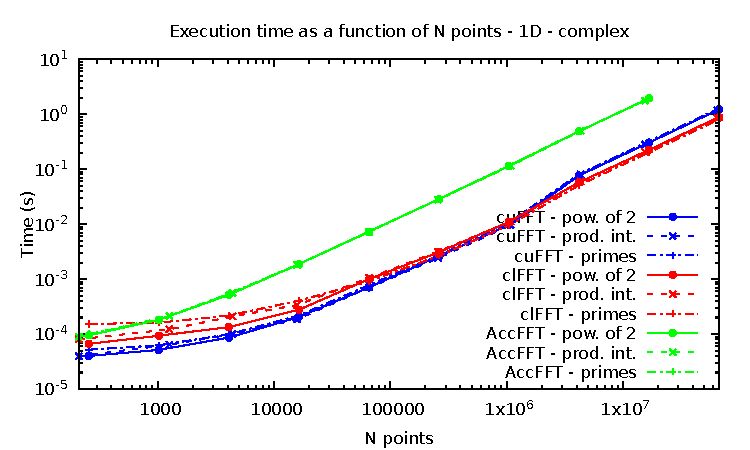
\includegraphics[width=.9\linewidth]{graphs/fft-1d-c-exec.pdf}
\caption{Intialisation (complex)}
\label{FFT1DCI}
\end{subfigure}%
\begin{subfigure}{.5\textwidth}
\centering
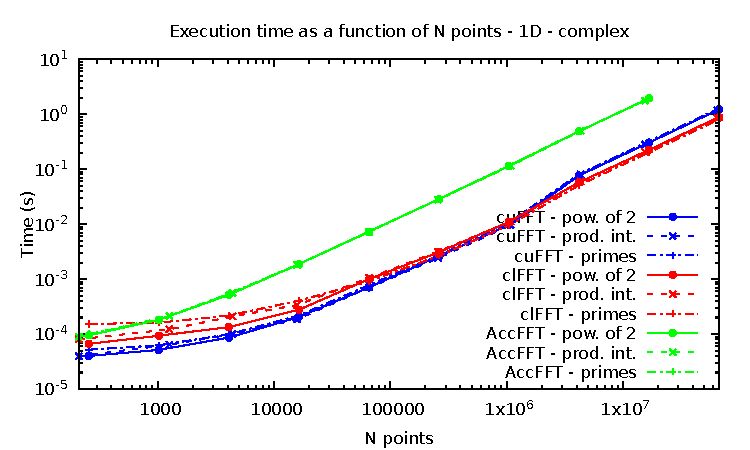
\includegraphics[width=.9\linewidth]{graphs/fft-1d-c-exec.pdf}
\caption{Execution (complex)}
\label{FFT1DCE}
\end{subfigure}
\caption{Initialisation and execution times as a function of the number of points (1 dimension)}
\label{FFT1D}
\end{figure}

\subsection{Effect of the domain size in two dimensions}\label{PERFORMANCE2D}
We repeat the analysis done in Section \ref{PERFORMANCE1D} but, this
time, in two dimensions, on a square domain. The sizes of the domain along one side
are given in table \ref{2DSIZES}.

\begin{table}[H]
\centering
\begin{tabular}{|l|l|l|}
  \hline
  \multicolumn{3}{|c|}{$N_x=N_y$}\\
  \hline
  \hline
Powers of 2 & prod. pow. int. & primes\\ \hline
$2^9 = 512$ & $2^3\ 3^2\ 7 = 504$ & 509\\ \hline
$2^{10} = 1024$ & $3\ 7^3 = 1029$ & 1021\\ \hline
$2^{11} = 2048$	& $2\ 3 \ 7^3 = 2058$ &	2027\\ \hline
$2^{12} = 4096$	& $2^2\ 3\ 7^3 = 4116$ & 4049\\ \hline
$2^{13} = 8192$	& $2^3\ 3\ 7^3 = 8232$ & 8123\\ \hline
\end{tabular}
\caption{Number of points (along one domain edge) used for the benchmark in two dimensions}\label{2DSIZES}
\end{table}

The libraries are compared in Figures~\ref{FFTPOW22D} and \ref{FFT2D}.
In two dimensions, clFFT performs slightly better than cuFFT while
AccFFT lags behind. However clFFT suffers from the same drawback as
the one we had identified in Section \ref{PERFORMANCE1D}. In most
cases, the performance tends to be worse when
the number of points on the side of the domain is a prime number
rather than a power of two or the product of powers of small
integers.



\begin{figure}[H]
\captionsetup{width=0.8\linewidth}
\centering
\begin{subfigure}{.5\textwidth}
\centering
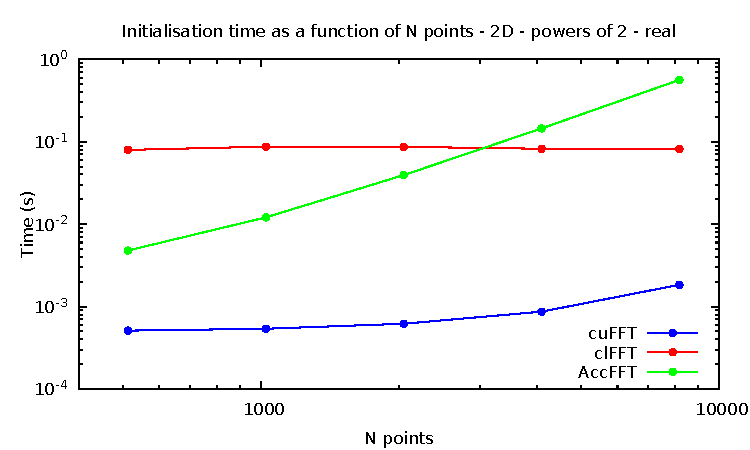
\includegraphics[width=.9\linewidth]{graphs/fft-2d-pow2-r-init.pdf}
\caption{Intialisation (real)}
\label{FFTPOW22DRI}
\end{subfigure}%
\begin{subfigure}{.5\textwidth}
\centering
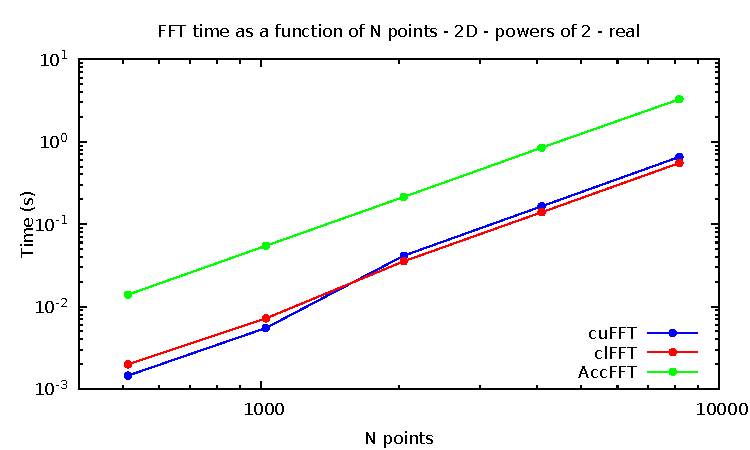
\includegraphics[width=.9\linewidth]{graphs/fft-2d-pow2-r-exec.pdf}
\caption{Execution (real)}
\label{FFTPOW22DRE}
\end{subfigure}\\
\begin{subfigure}{.5\textwidth}
\centering
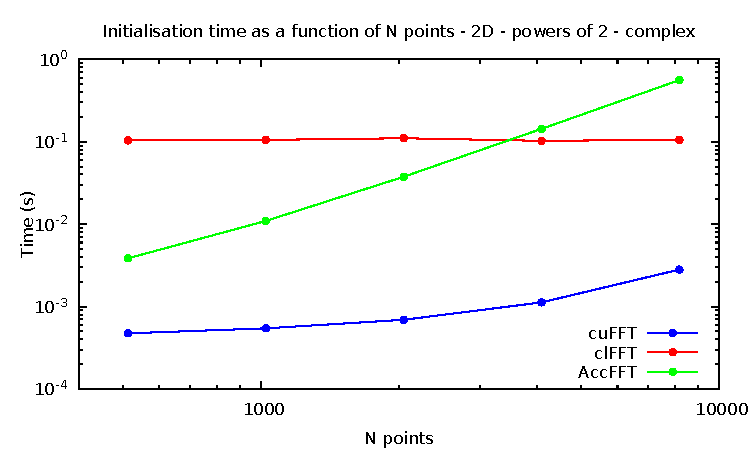
\includegraphics[width=.9\linewidth]{graphs/fft-2d-pow2-c-init.pdf}
\caption{Intialisation (complex)}
\label{FFTPOW22DCI}
\end{subfigure}%
\begin{subfigure}{.5\textwidth}
\centering
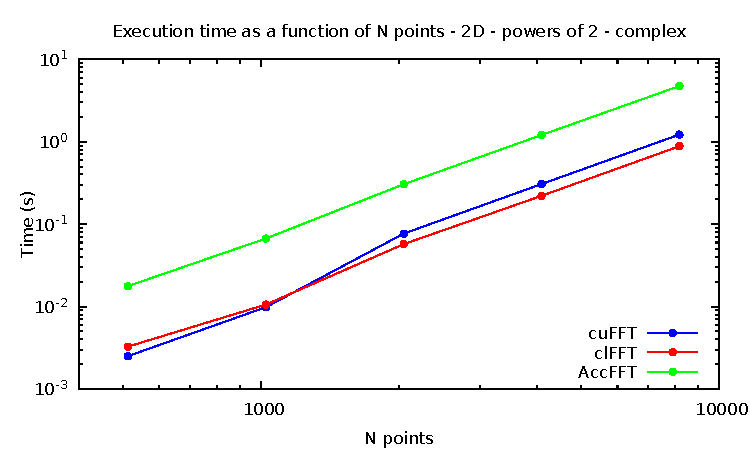
\includegraphics[width=.9\linewidth]{graphs/fft-2d-pow2-c-exec.pdf}
\caption{Execution (complex)}
\label{FFTPOW22DCE}
\end{subfigure}
\caption{Initialisation and execution times as a function of the number of points (2 dimensions, powers of 2)}
\label{FFTPOW22D}
\end{figure}

\begin{figure}[H]
\captionsetup{width=0.8\linewidth}
\centering
\begin{subfigure}{.5\textwidth}
\centering
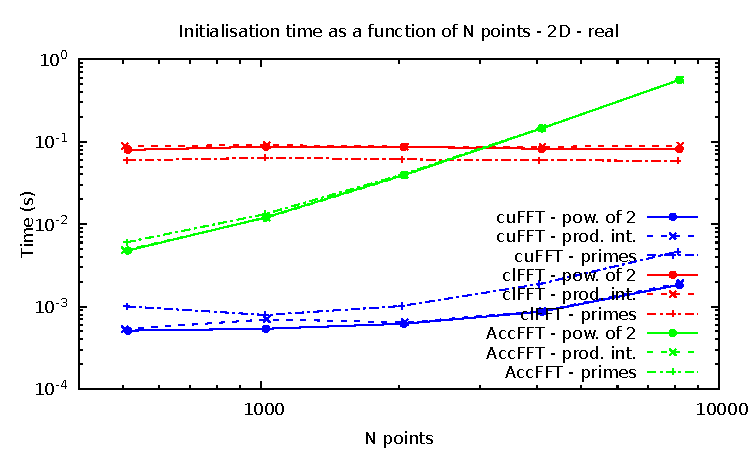
\includegraphics[width=.9\linewidth]{graphs/fft-2d-r-init.pdf}
\caption{Intialisation (real)}
\label{FFT2DRI}
\end{subfigure}%
\begin{subfigure}{.5\textwidth}
\centering
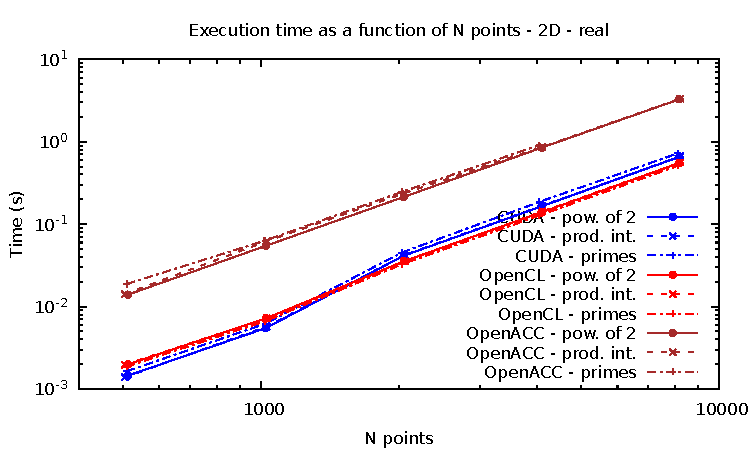
\includegraphics[width=.9\linewidth]{graphs/fft-2d-r-exec.pdf}
\caption{Execution (real)}
\label{FFT2DRE}
\end{subfigure}\\
\begin{subfigure}{.5\textwidth}
\centering
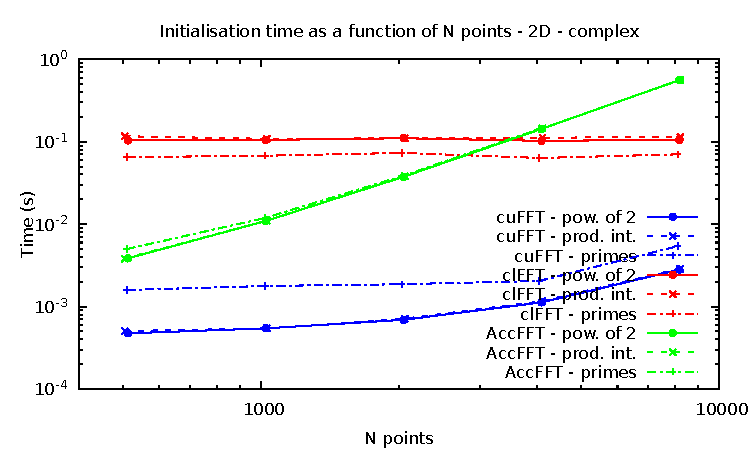
\includegraphics[width=.9\linewidth]{graphs/fft-2d-c-init.pdf}
\caption{Intialisation (complex)}
\label{FFT2DCI}
\end{subfigure}%
\begin{subfigure}{.5\textwidth}
\centering
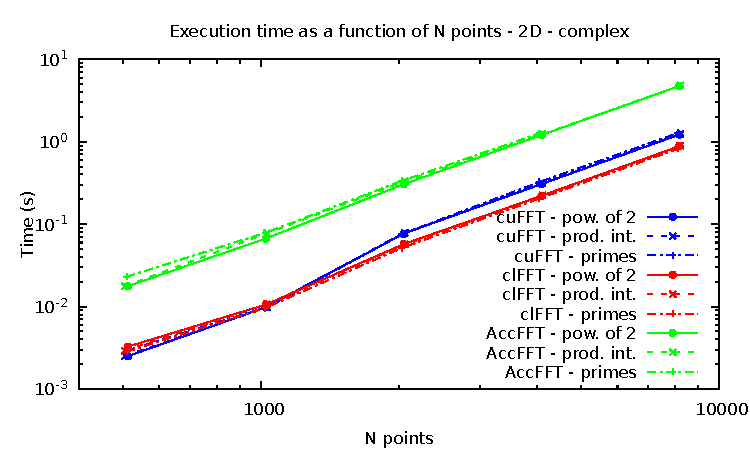
\includegraphics[width=.9\linewidth]{graphs/fft-2d-c-exec.pdf}
\caption{Execution (complex)}
\label{FFT2DCE}
\end{subfigure}
\caption{Initialisation and execution times as a function of the number of points (2 dimensions)}
\label{FFT2D}
\end{figure}


\subsection{Effect of the domain size in three dimensions}\label{PERFORMANCE3D}
After having assessed the performance obtained in one (Section
\ref{PERFORMANCE1D}) and two (Section \ref{PERFORMANCE3D}) dimensions,
we measure it in three dimensions, on a cubic domain whose sizes are
given in Table~\ref{3DSIZES}.

\begin{table}[H]
  \centering
  \captionsetup{width=0.8\linewidth}
\begin{tabular}{|l|l|l|}
  \hline
  \multicolumn{3}{|c|}{$N_x=N_y=N_z$}\\
  \hline
  \hline
Powers of 2 & prod. pow. int. & primes\\ \hline
$2^5 = 32$ & $2\times 3\times 5 =	30$ & 31\\ \hline
$2^6 = 64$ & $2\times 5\times 7 = 70$ & 61\\ \hline
$2^7 = 128$ & $3\times 5\times 7 = 105$ & 127\\ \hline
$2^8 = 256$ & $2\times 3\times 5\times 7 = 210$ & 257\\ \hline
$2^9 = 512$ & $2^2\times 3\times 5\times 7 = 420$ & 509\\ \hline
\end{tabular}
\caption{Number of points used for the benchmark in three dimensions}\label{3DSIZES}
\end{table}

We compare the libraries in Figures~\ref{FFTPOW23D} and \ref{FFT3D}.
In three dimensions, clFFT and cuFFT exhibit performances that are
close and they are both significantly faster than AccFFT. However,
for large domains, clFFT performs slightly better. Unfortunately, it
is plagued by the problem we identified in the previous section: its
initialisation time is quite long and does not decrease with the
number of points. Finally, we do not observe any large difference
between the performance obtained when the sides of the domain are a
power of two, the product of powers of small integers or a prime
number.



\begin{figure}[H]
\captionsetup{width=0.8\linewidth}
\centering
\begin{subfigure}{.5\textwidth}
\centering
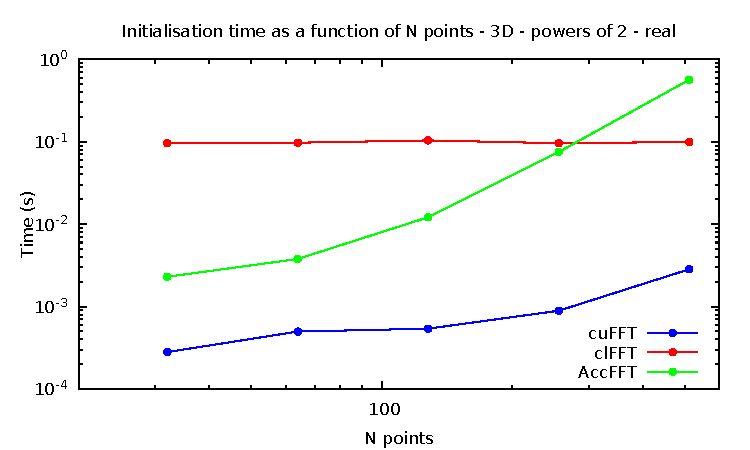
\includegraphics[width=.9\linewidth]{graphs/fft-3d-pow2-r-init.pdf}
\caption{Intialisation (real)}
\label{FFTPOW23DRI}
\end{subfigure}%
\begin{subfigure}{.5\textwidth}
\centering
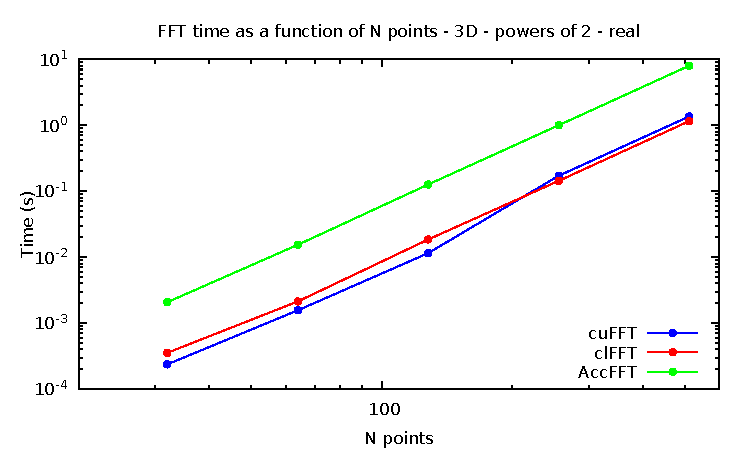
\includegraphics[width=.9\linewidth]{graphs/fft-3d-pow2-r-exec.pdf}
\caption{Execution (real)}
\label{FFTPOW23DRE}
\end{subfigure}\\
\begin{subfigure}{.5\textwidth}
\centering
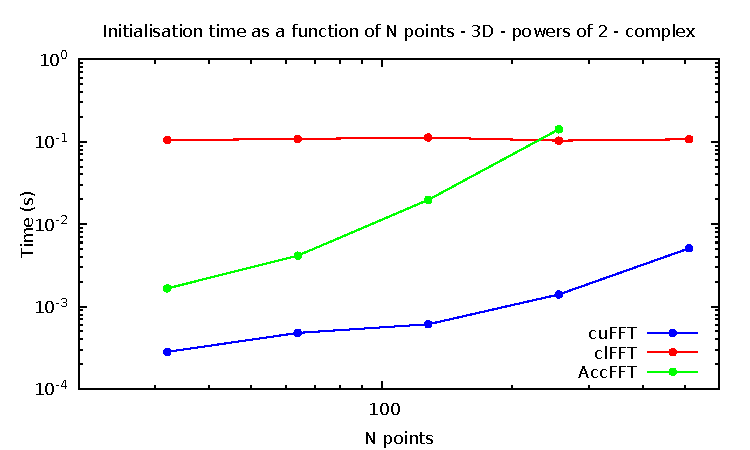
\includegraphics[width=.9\linewidth]{graphs/fft-3d-pow2-c-init.pdf}
\caption{Intialisation (complex)}
\label{FFTPOW23DCI}
\end{subfigure}%
\begin{subfigure}{.5\textwidth}
\centering
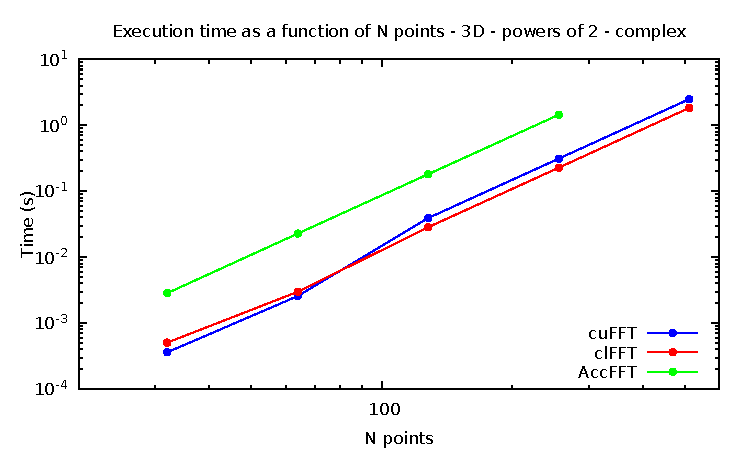
\includegraphics[width=.9\linewidth]{graphs/fft-3d-pow2-c-exec.pdf}
\caption{Execution (complex)}
\label{FFTPOW23DCE}
\end{subfigure}
\caption{Initialisation and execution times as a function of the number of points (3 dimensions, powers of 2)}
\label{FFTPOW23D}
\end{figure}

\begin{figure}[H]
\captionsetup{width=0.8\linewidth}
\centering
\begin{subfigure}{.5\textwidth}
\centering
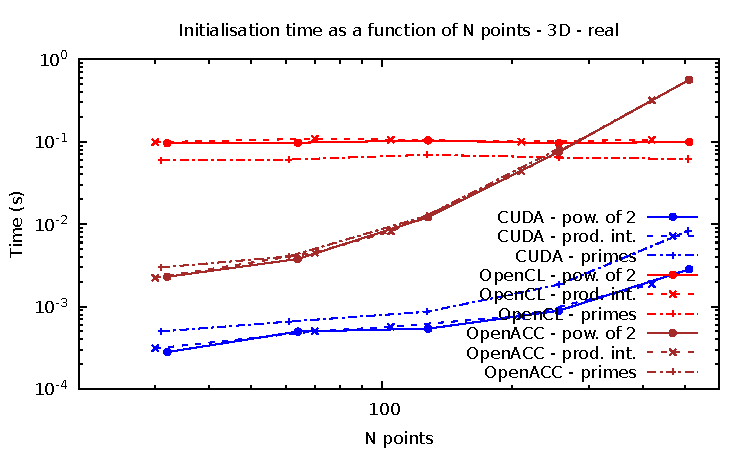
\includegraphics[width=.9\linewidth]{graphs/fft-3d-r-init.pdf}
\caption{Intialisation (real)}
\label{FFT3DRI}
\end{subfigure}%
\begin{subfigure}{.5\textwidth}
\centering
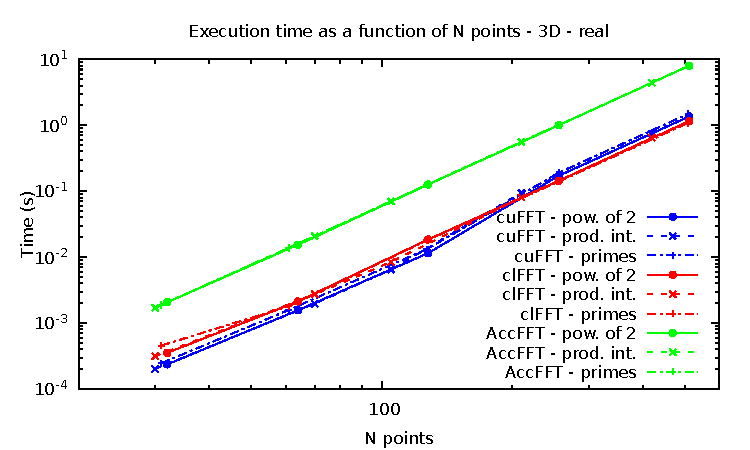
\includegraphics[width=.9\linewidth]{graphs/fft-3d-r-exec.pdf}
\caption{Execution (real)}
\label{FFT3DRE}
\end{subfigure}\\
\begin{subfigure}{.5\textwidth}
\centering
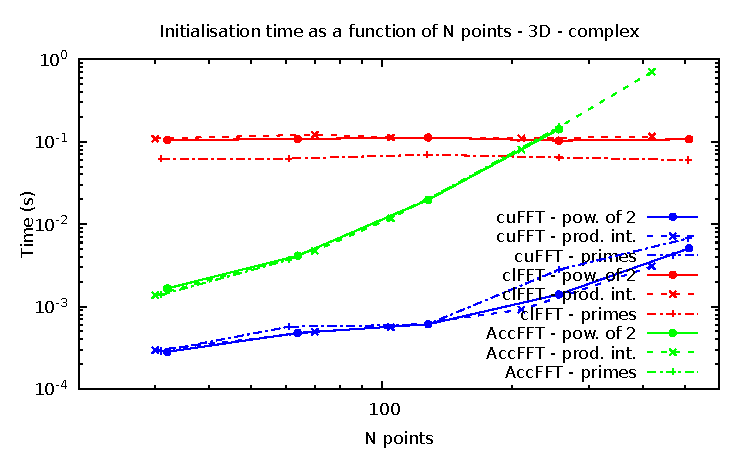
\includegraphics[width=.9\linewidth]{graphs/fft-3d-c-init.pdf}
\caption{Intialisation (complex)}
\label{FFT3DCI}
\end{subfigure}%
\begin{subfigure}{.5\textwidth}
\centering
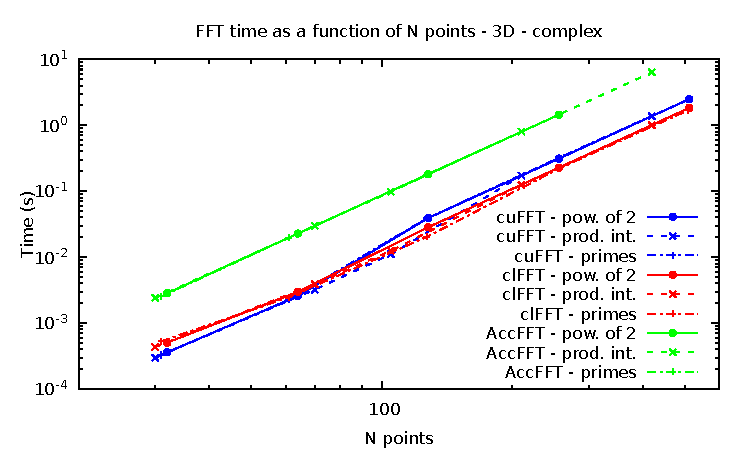
\includegraphics[width=.9\linewidth]{graphs/fft-3d-c-exec.pdf}
\caption{Execution (complex)}
\label{FFT3DCE}
\end{subfigure}
\caption{Initialisation and execution times as a function of the number of points (3 dimensions)}
\label{FFT3D}
\end{figure}

\subsection{Flatness}\label{FLATNESS}
So far, we have considered only square or cubic domains. In this
section, we study the effect of the flatness of the domain by
computing the FFT on an increasingly flat cuboid containing $256^3$
points. We define the flatness by the ratio between the number of
points in the $z$ and $x$ directions whereas the dimensions in the $x$
and $y$ directions are identical (Flatness:=$N_z/N_x$, $N_x=N_y$)
(Table~\ref{FLATNESSDIM}).

\begin{table}[H]
\centering
\begin{tabular}{|l|l|l|}
\hline
$N_x=N_y$ & $N_z $ & Flatness\\ 
\hline
\hline
256 & 256 & 1\\ \hline
128 & 1024 & 8\\ \hline
64 & 4096 & 64\\ \hline
32 & 16384 & 512\\ \hline
16 & 65536 & 4096\\ \hline
8 & 262144 & 32768\\ \hline
4 & 1048576 & 262144\\ \hline 
2 & 4194304 & 2097152\\ \hline
\end{tabular}
\caption{Number of points used for the benchmark in three dimensions}\label{FLATNESSDIM}
\end{table}

We observe that the flatness does not alter significantly the
performance which remains dependent only on the total number of
points.

\begin{figure}[H]
\captionsetup{width=0.8\linewidth}
\centering
\begin{subfigure}{.5\textwidth}
\centering
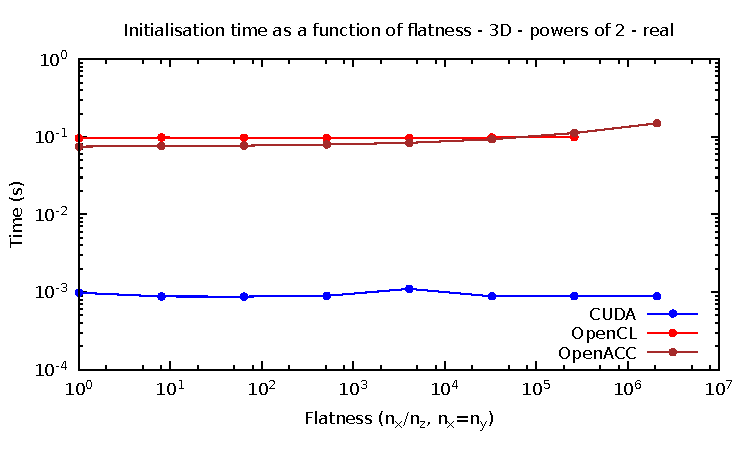
\includegraphics[width=.9\linewidth]{graphs/flatness-r-init.pdf}
\caption{Intialisation (real)}
\label{FLAT1DRI}
\end{subfigure}%
\begin{subfigure}{.5\textwidth}
\centering
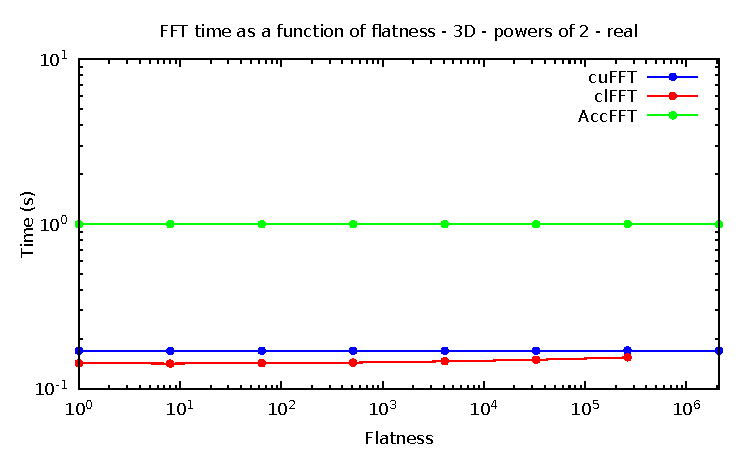
\includegraphics[width=.9\linewidth]{graphs/flatness-r-exec.pdf}
\caption{Execution (real)}
\label{FLAT1DRE}
\end{subfigure}\\
\begin{subfigure}{.5\textwidth}
\centering
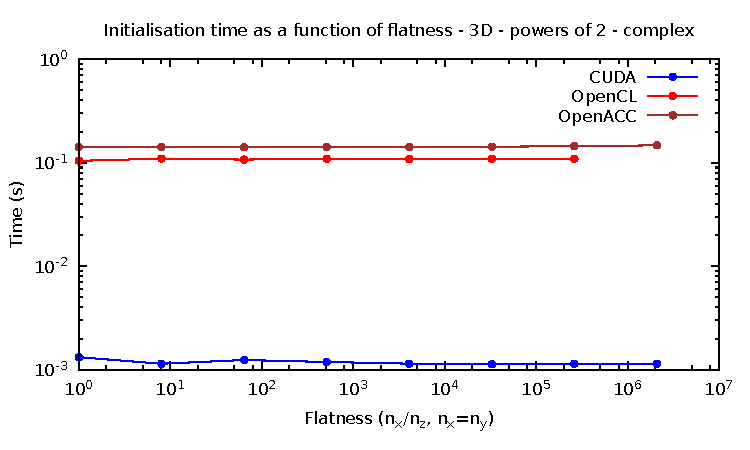
\includegraphics[width=.9\linewidth]{graphs/flatness-c-init.pdf}
\caption{Intialisation (complex)}
\label{FLAT1DCI}
\end{subfigure}%
\begin{subfigure}{.5\textwidth}
\centering
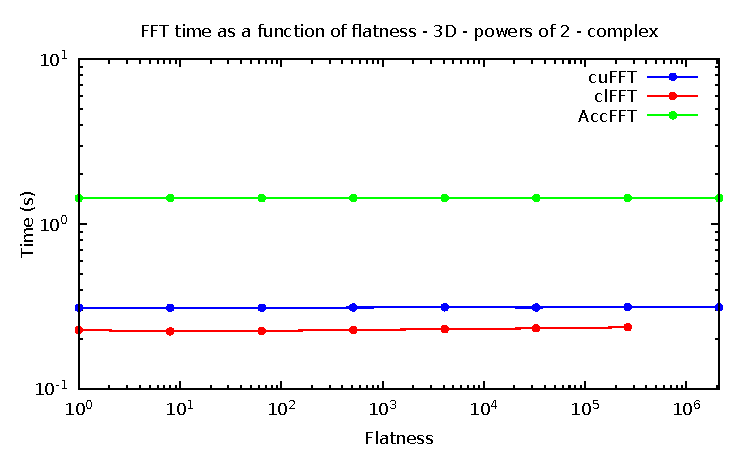
\includegraphics[width=.9\linewidth]{graphs/flatness-c-exec.pdf}
\caption{Execution (complex)}
\label{FLAT1DCE}
\end{subfigure}
\caption{Initialisation and execution times as a function of the flatness ($N_z/N_x$, $N_x=N_y$) of the domain (3 dimensions)}
\label{FLATNESSGRAPH}
\end{figure}

\subsection{Requirements from the CCP}\label{CCPPETMR}
We have also benchmarked the libraries provided by these frameworks
for the computation of FFTs in a context similar to the situation
encountered by the CCP/PET-MR collaboration. In this example, we
compute the FFT of 32 square complex images. Their side is made of
252, 256 and 257 points in the cases, respectively, of a number of
points corresponding to a product of powers of small integers, a power
of 2 or a prime number. In this context, it is cuFFT that is the most
efficient.
\begin{figure}[H]
\captionsetup{width=0.8\linewidth}
\centering
\begin{subfigure}{.5\textwidth}
\centering
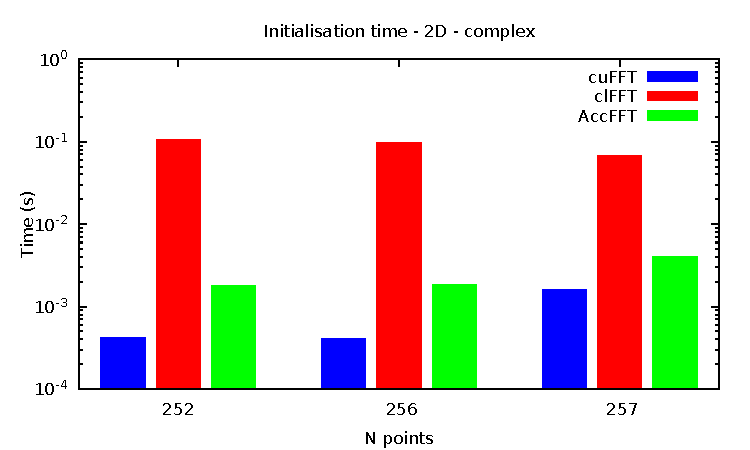
\includegraphics[width=.9\linewidth]{graphs/fft-ccppetmr-init.pdf}
\caption{Intialisation (real)}
\label{CCPPETMRDRI}
\end{subfigure}%
\begin{subfigure}{.5\textwidth}
\centering
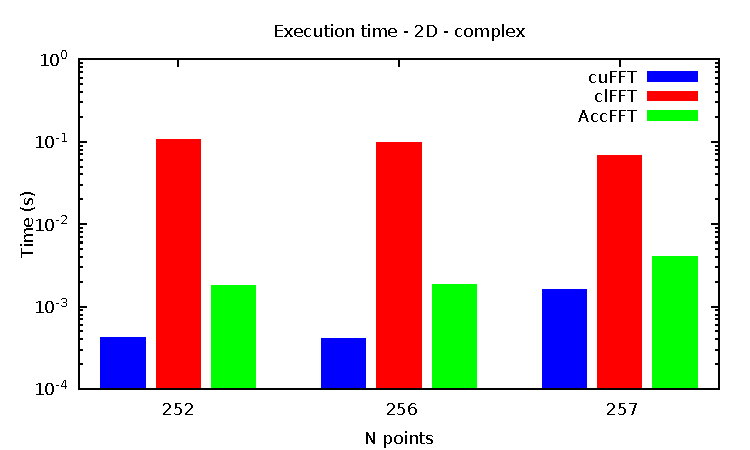
\includegraphics[width=.9\linewidth]{graphs/fft-ccppetmr-exec.pdf}
\caption{Execution (real)}
\label{CCPPETMRRE}
\end{subfigure}
\caption{Initialisation and execution times as a function of the number of points (3 dimensions)}
\label{CCPPETMRGRAPH}
\end{figure}

\section{Conclusion}
For the execution on the GPU of a small piece of code we have
programmed, OpenMP was the most efficient framework. In the case of
the computation of a FFT using a library, CUDA's cuFFT and clFFT's
clFFT offer performances that are close in terms of wallclock FFT
execution time but cuFFT's initialisation times were much lower than
thos of clFFT. As a consequence, the library provided by CUDA seems
the most efficient. We also note that frameworks based on preprocessor
directives, such as OpenMP and OpenACC, are much easier to use.

\section*{Acknowledgements}
This work made use of computational support by CoSeC, the
Computational Science Centre for Research Communities, through its
Software Outlook activity.

\begin{thebibliography}{9}

\bibitem{cuda} CUDA Toolkit from NVIDIA, \url{https://developer.nvidia.com/cuda-zone}

\bibitem{opencl} OpenCL (Open Computing Language, \url{https://www.khronos.org/opencl/}

\bibitem{openacc} OpenACC, \url{https://www.openacc.org/}
  
\bibitem{openmp} OpenMP, \url{https://www.openmp.org/}

\bibitem{kokkos} Kokkos C++ Performance Portability Programming EcoSystem,
\url{https://github.com/kokkos}

\bibitem{cufft} CUDA Fast Fourier Transform library, cuFFT, \url{https://docs.nvidia.com/cuda/cufft/index.html}

\bibitem{clfft} The ACL clFFT Library, \url{https://github.com/clMathLibraries/clFFT}
  
\bibitem{accfft} AccFFT: A Massively Parallel FFT Library for CPU/GPU, \url{http://accfft.org/}

\bibitem{ccppetmr} CCP PET-MR, Collaborative Computational Project in Positron Emission Tomography and Magnetic Resonance imaging, \url{https://www.ccppetmr.ac.uk/}

\bibitem{softwareoutlook} Software Outlook, \url{https://www.softwareoutlook.ac.uk/}

\bibitem{FFTREPORT}  Gambron, P., Thorne, H. S.,
{\it Comparison of FFT libraries for use in C/C++ codes}, Tech. Rep. RAL-TR-2020-XX, 2020.

\bibitem{KOKKOSDOC} Kokkos: Compiling, \url{https://github.com/kokkos/kokkos/wiki/Compiling}

\end{thebibliography}

\end{document}
